Let $G(V, E, w)$ represent an undirected graph, where $V$ denotes the set of vertices, $E$ denotes the set of edges, and $w_{ij} = w_{ji}$ signifies a positive weight associated with each edge in the graph. In the case of an unweighted graph, we assume each edge has a unit weight ($w_{ij} = 1$). Additionally, we denote the neighbors of each vertex $i$ as $J_i = \{j\ |\ (i, j) \in E\}$, the weighted degree of each vertex $i$ as $K_i = \sum_{j \in J_i} w_{ij}$, the total number of vertices in the graph as $N = |V|$, the total number of edges in the graph as $M = |E|$, and the sum of edge weights in the undirected graph as $m = \sum_{i, j \in V} w_{ij}/2$.




\subsection{Community detection}

Disjoint community detection involves finding a community membership mapping, $C: V \rightarrow \Gamma$, which maps each vertex $i \in V$ to a community ID $c \in \Gamma$, where $\Gamma$ is the set of community-ids. The vertices within a community $c$ are denoted as $V_c$, and the community to which a vertex $i$ belongs is denoted as $C_i$. Furthermore, we define the neighbors of vertex $i$ belonging to a community $c$ as $J_{i \rightarrow c} = \{j\ |\ j \in J_i\ and\ C_j = c\}$, the sum of those edge weights as $K_{i \rightarrow c} = \{w_{ij}\ |\ j \in J_{i \rightarrow c}\}$, the sum of edge weights within $c$ as $\sigma_c = \sum_{(i, j) \in E\ and\ C_i = C_j = c} w_{ij}$, and the total edge weight of $c$ as $\Sigma_c = \sum_{(i, j) \in E\ \mbox{and}\ C_i = c} w_{ij}$ \cite{com-zarayeneh21}.




\subsection{Modularity}

Modularity is a metric used to assess the quality of communities identified by community detection algorithms, which are\ignore{typically} heuristic-based \cite{com-newman04}. It ranges from $[-0.5, 1]$ (higher is better), and is calculated as the difference between the fraction of edges within communities and the expected fraction of edges if they were distributed randomly \cite{com-brandes07}.\ignore{Theoretically, optimizing this function leads to the best possible grouping\ignore{ of the network} \cite{com-newman04, com-traag11}.} The modularity $Q$ of the obtained communities can be calculated using Equation \ref{eq:modularity}\ignore{, where $\delta$ represents the Kronecker delta function ($\delta (x,y)=1$ if $x=y$ and $0$ otherwise)}. The \textit{delta modularity} of moving a vertex $i$ from community $d$ to community $c$, denoted as $\Delta Q_{i: d \rightarrow c}$, is determined using Equation \ref{eq:delta-modularity}.


\begin{equation}
\label{eq:modularity}
  Q
  % = \frac{1}{2m} \sum_{(i, j) \in E} \left[w_{ij} - \frac{K_i K_j}{2m}\right] \delta(C_i, C_j)
  = \sum_{c \in \Gamma} \left[\frac{\sigma_c}{2m} - \left(\frac{\Sigma_c}{2m}\right)^2\right]
\end{equation}

\begin{equation}
\label{eq:delta-modularity}
  \Delta Q_{i: d \rightarrow c}
  = \frac{1}{m} (K_{i \rightarrow c} - K_{i \rightarrow d}) - \frac{K_i}{2m^2} (K_i + \Sigma_c - \Sigma_d)
\end{equation}




\subsection{Louvain algorithm}
\label{sec:about-Louvain}

The Louvain method is a greedy, modularity optimization based agglomerative algorithm for detecting communities of high quality in a graph. It works in two phases: in the local-moving phase, each vertex $i$ considers moving to a neighboring community $C_j\ |\ j \in J_i$ to maximize modularity increase $\Delta Q_{i:C_i \rightarrow C_j}$. In the aggregation phase, vertices in the same community are merged into super-vertices. These phases constitute a pass, and repeat until modularity gain stops. This produces a hierarchical structure (dendrogram), with the top level representing the final communities.
% As mentioned earlier, the Louvain method is a greedy, modularity optimization-based agglomerative algorithm that identifies high-quality communities within a graph \cite{com-lancichinetti09}. The method operates in two phases\ignore{: the local-moving phase and the aggregation phase}. In the local-moving phase, each vertex $i$ evaluates moving to the community of one of its neighbors $j \in J_i$ that maximizes the increase in modularity $\Delta Q_{i:C_i \rightarrow C_j}$ (using Equation \ref{eq:delta-modularity}). In the aggregation phase, all vertices within the same community are collapsed into a super-vertex. These two phases constitute one pass, which is repeated until there is no further gain in modularity. The method produces a hierarchy of community memberships for each vertex, forming a dendrogram, with the top-level\ignore{hierarchy} representing the final communities.



\subsection{Leiden algorithm}
\label{sec:about-leiden}

As previously mentioned, the Louvain method, while effective, can produce internally disconnected or poorly connected communities. To address these issues, Traag et al. \cite{com-traag19} proposed the Leiden algorithm. This algorithm introduces a \textit{refinement phase} following the local-moving phase. During this phase, vertices within each community undergo constrained merges into other sub-communities within their community bounds (established during the local moving phase), starting from a singleton sub-community. This process is randomized, with the probability of a vertex joining a neighboring sub-community being proportional to the delta-modularity of the move. This step helps identify sub-communities within those identified during the local-moving phase. The Leiden algorithm ensures that all communities are well-separated and well-connected. Once the communities have converged, it guarantees that all vertices are optimally assigned and all communities are subset optimal \cite{com-traag19}. The Leiden algorithm has a time complexity of $O(L|E|)$, where $L$ is the total number of iterations performed, and a space complexity of $O(|V| + |E|)$, similar to the Louvain method.
% which each pass consisting of local-moving, refinement, and aggregation phases




\subsection{Dynamic approaches}
\label{sec:dynamic-graphs}

A dynamic graph can be represented as a sequence of graphs, where $G^t(V^t, E^t, w^t)$ denotes the graph at time step $t$. The changes between the graphs $G^{t-1}(V^{t-1}, E^{t-1}, w^{t-1})$ and $G^t(V^t, E^t, w^t)$ at consecutive time steps $t-1$ and $t$ can be described as a batch update $\Delta^t$ at time step $t$. This batch update consists of a set of edge deletions $\Delta^{t-} = \{(i, j)\ |\ i, j \in V\} = E^{t-1} \setminus E^t$ and a set of edge insertions $\Delta^{t+} = \{(i, j, w_{ij})\ |\ i, j \in V; w_{ij} > 0\} = E^t \setminus E^{t-1}$ \cite{com-zarayeneh21}. We refer to the scenario where $\Delta^t$ includes multiple edges being deleted and inserted as a \textit{batch update}.


\subsubsection{Naive-dynamic (ND) approach \cite{com-aynaud10, com-chong13, com-shang14, com-zhuang19}}
\label{sec:naive-dynamic}

The Naive dynamic approach\ignore{, presented by Aynaud et al. \cite{com-aynaud10},} is a simple method for detecting communities in dynamic networks. In this approach, vertices are assigned to communities based on the previous snapshot of the graph, and all vertices are processed, regardless of the edge deletions and insertions in the batch update (hence the term \textit{naive}).
% This is illustrated in Figure \ref{fig:about-cases--naive}, where all vertices are marked as affected and highlighted in yellow. As all communities are also marked as affected, they are depicted with hatching. In the figure, edge deletions are shown in the top row (indicated by dotted lines), edge insertions are shown in the middle row (also indicated by dotted lines), and vertex migration during the community detection algorithm is shown in the bottom row. The community membership obtained through this method is guaranteed to be at least as accurate as that obtained by the static algorithm.


\subsubsection{Delta-screening (DS) approach \cite{com-zarayeneh21}}
\label{sec:delta-screening}

This is a dynamic community detection approach that utilizes modularity-based scoring to identify an approximate region of the graph where vertices are likely to alter their community membership. In the DS approach, Zarayeneh et al. first sort the batch update consisting of edge deletions $(i, j) \in \Delta^{t-}$ and insertions $(i, j, w) \in \Delta^{t+}$ by their source vertex ID. For edge deletions within the same community, they mark $i$'s neighbors and $j$'s community as affected. For edge insertions across communities, they select the vertex $j^*$ with the highest modularity change among all insertions linked to vertex $i$ and mark $i$'s neighbors and $j^*$'s community as affected. Edge deletions between different communities and edge insertions within the same community are unlikely to impact community membership and are therefore ignored. Figure \ref{fig:about-cases--delta} shows the vertices (and communities) connected to a single source vertex $i$ that are identified as affected by the DS approach, in response to a batch update with both edge deletions and insertions.


\subsubsection{Dynamic Frontier (DF) approach \cite{sahu2024shared}}
\label{sec:about-frontier}

This approach first initializes each vertex's community membership to that obtained in the previous graph snapshot. In instances where edge deletions occur between vertices within the same community or edge insertions between vertices in different communities, the DF approach marks the source vertex $i$ as affected\ignore{, as depicted by the yellow-highlighted vertices in Figure \ref{fig:about-cases--frontier}}. As batch updates are undirected, both endpoints $i$ and $j$ are effectively marked as affected. Edge deletions spanning different communities or edge insertions within the same community are disregarded (as previously mentioned in Section \ref{sec:delta-screening}). Furthermore, when a vertex $i$ alters its community membership during the community detection process\ignore{(illustrated by $i$ transitioning from its original community in the center to its new community on the right)}, all its neighboring vertices $j \in J_i$ are marked as affected\ignore{, as depicted in Figure \ref{fig:about-cases--frontier} (highlighted in yellow)}, while $i$ is marked as unaffected. To minimize unnecessary computation, an affected vertex $i$ is also marked as unaffected even if its community remains unchanged. Thus, the DF approach follows a graph traversal-like process until the vertices' community assignments converge. Figure \ref{fig:about-cases--frontier} shows vertices connected to a single source vertex $i$ identified as affected by the DF approach in response to a batch update.
% When processing a batch update containing edge deletions $(i, j, w) \in \Delta^{t-}$ and insertions $(i, j, w) \in \Delta^{t+}$ upon the original graph, it is likely that only a small subset of vertices in the graph would undergo a change in their community membership. However, the ND approach processes all vertices, while the DS approach tends to overestimate the set of affected vertices, while incurring a high overhead in estimating the set of affected vertices.
% This optimization, referred to as vertex pruning \cite{com-ozaki16, com-ryu16, com-shi21, com-zhang21}.

\begin{figure}[hbtp]
  \centering
  % \subfigure[Naive-dynamic (ND) approach]{
  %   \label{fig:about-cases--naive}
  %   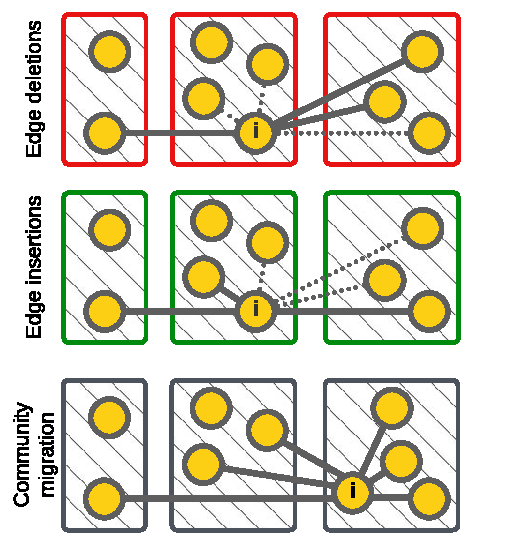
\includegraphics[width=0.3\linewidth]{out/about-cases-naive.pdf}
  % }
  \subfigure[Delta-screening (DS)]{
    \label{fig:about-cases--delta}
    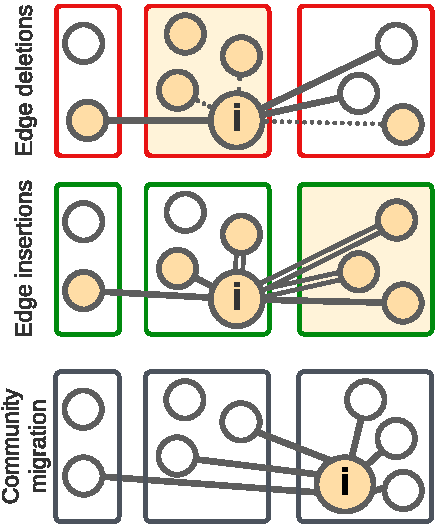
\includegraphics[width=0.468\linewidth]{out/about-cases-delta.pdf}
  }
  \subfigure[Dynamic Frontier (DF)]{
    \label{fig:about-cases--frontier}
    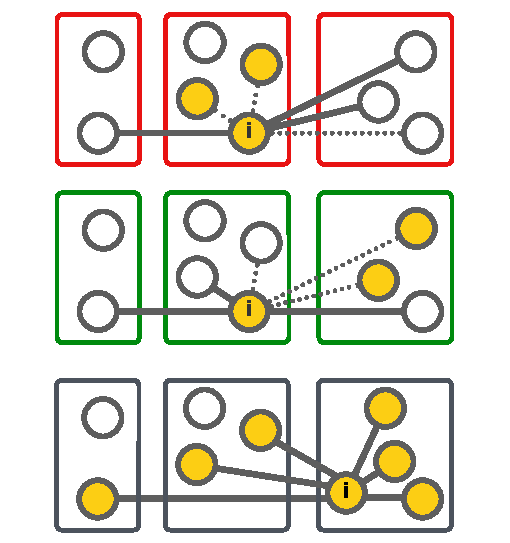
\includegraphics[width=0.43\linewidth]{out/about-cases-frontier.pdf}
  } \\[-1ex]
  \caption{Illustration of \textit{Delta-screening (DS)} \cite{com-zarayeneh21} and \textit{Dynamic Frontier (DF)} approaches \cite{sahu2024shared}, in the presence of edge deletions and insertions, represented with dotted lines and doubled lines, respectively. Vertices identified as affected (initial) by each approach are highlighted in brown, and entire communities marked as affected are depicted in light brown.}
  \label{fig:about-cases}
\end{figure}

